\documentclass{bioinfo}
\usepackage{url}

\usepackage[british,english]{babel}
\usepackage{mathpazo}
\usepackage[T1]{fontenc}
% \usepackage[latin9]{inputenc}
\usepackage{float}
\usepackage{amsmath}
\usepackage{graphicx}
\usepackage{setspace}
\usepackage{amssymb}
\usepackage{natbib}
\usepackage[title]{appendix}
\usepackage{siunitx}
\usepackage{chngcntr}
\usepackage{algorithmic}
\usepackage{listings}
\usepackage{multicol}
\usepackage{widetext}
\renewcommand{\algorithmicrequire}{\textbf{Input:}}
\renewcommand{\algorithmicensure}{\textbf{Output:}}

\usepackage{multirow}
\usepackage{rotating}

\graphicspath{{Figures/}}

\lstset{language=python,
	basicstyle=\ttfamily,
	extendedchars=true,
	xleftmargin = 0pt,
	% rulecolor=\color{black!50},
        aboveskip = 0.5ex,
        belowskip = 0.6ex,
	%escapebegin={\color{green!50!black}},
	%commentstyle=\slshape\color{green!50!black},
	%stringstyle=\rmfamily\color{blue},
	showstringspaces=false,
	tabsize=2,
	breaklines=true,
        morekeywords={{,},=,:},
        frame=single,xleftmargin=\fboxsep,xrightmargin=-\fboxsep
    }


\makeatletter
\newfloat{algorithm}{H}{loa}[section]
\floatname{algorithm}{Algorithm}
\counterwithout{algorithm}{algorithm}
\def\argmin{\mathop{\operator@font arg\,min}} 
\def\argmax{\mathop{\operator@font arg\,max}} 
\makeatother

\copyrightyear{}
\pubyear{}

\begin{document}
\firstpage{1}

\title[nipy-paper]{Analysis of functional imaging data with NIPY}

% Alexis Roche1, Bertrand Thirion2, Gael Varoquaux2, Jonathan Taylor3, Matthew Brett4 and nipy contributors5
% 
% 1. University Hospital Lausanne/Siemens Medical Solutions, CIBM, Lausanne, Switzerland
% 2. Neurospin, CEA Saclay, Gif sur Yvette, France
% 3. Stanford University, Stanford, CA, USA,
% 4. University of California, Berkeley, CA, USA,
% 5. https://github.com/nipy/nipy/contributors

\author[Roche,Thirion,Varoquaux,Taylor,Brett]{Alexis~Roche\,$^{1,2}$,
  Bertrand~Thirion\,$^{3}$, Ga\"el~Varoquaux\,$^{3}$,
  Jonathan~Taylor\,$^{4}$, Matthew~Brett\,$^{5} \footnote{to whom
    correspondence should be addressed. e-mail:
    matthew.brett@gmail.com}$, and NIPY contributors}

\address{\,$^{1}$University Hospital, Lausanne, Switzerland\\
  \,$^{2}$Siemens Healthcare Sector, Lausanne, Switzerland\\ 
  \,$^{3}$INRIA, Parietal team, Neurospin, Saclay, France\\
  \,$^{4}$Stanford University, Stanford, CA, USA\\
  \,$^{5}$University of California, Berkeley, CA, USA}


\history{}

\editor{}

\maketitle

\begin{abstract}
\noindent

NIPY is a library and application for analysing functional imaging data.   We
intended the project to be a project open to anyone who wanted to contribute
high-quality code.  Our aim is to make it easier for researchers to understand
the analysis and build their own tools, by writing code that is clear,
well-adapted to the scientific problem, and fast enough to run in reasonable
time.

Using Python has made it easier for us to work together because of the
readability of the language, the popularity of the language among
open-source developers, and Python's emphasis on testing and
documentation.

The package developed from a collaboration between researchers in Stanford,
Berkeley and CEA Neurospin in France.

Notable features of the NIPY package are: scriptable image diagnostics
including flexible PCA; combined slice-timing and movement correction
for functional MRI images; flexible registration model with pluggable
cost functions and optimization algorithms; common spatial models of
function encountered in neuroimaging (cluster-level models;
parcellations); fast and flexible specification of regression models
within and across subjects and groups; visualization of statistical
brain maps in 2D and 3D.

We will describe these features of the package with examples of their use.

\section{Keywords:} Python, functional MRI, structural MRI, 
Deconvolution, Medical imaging, Open source software, Deterministic
tractography, Probabilistic tractography, Visualisation.

\end{abstract}

\section*{Skeleton}

This section will be removed later on. Let's have it for now to
clarify the paper outline for every author. Here is a possible
outline, please feel free to modify:

\begin{verbatim}
Introduction
  Philosophy/Mission
  General Design Aspects
File Formats 
Preprocessing
   Image diagnostics
   Spatiotemporal realignment
   Generic image registration
Statistical analysis
   GLM specification/estimation
   Cluster-level analysis
   Parcel-based Bayesian analysis
Visualization
Conclusions
\end{verbatim}

\section{Introduction}

Someone will write this.

\section{File formats}

\section{Preprocessing}

\subsection{Image diagnostics}

\subsection{Spatiotemporal realignment}

FMRI sequences present spatio-temporal distortion due to the
combination of head motion during scanning and staggered slice
acquisition. While most fMRI processing packages provide tools to
correct for motion and slice timing separately, a common dilemma is to
determine which correction should be applied first. NIPY proposes a
four-dimensional realignment algorithm to perform both tasks
simultaneously \citep{roche:tmi:11}. This approach makes it possible
to account and correct for {\em continuous} movements that occur
throughout image acquisition. In addition, the method limits the
effect of BOLD signal changes on realignment \citep{freire:ni:01} by
using an adaptive reference image.

Spatiotemporal registration is implemented by a class called {\tt
  SpaceTimeRealign} which takes as initialization arguments a list of
four-dimensional images corresponding to successive fMRI runs for a
particular subject, and image acquisition information (inter-scan
repetition time, slice acquisition times, acquisition plane). Rigid
motion estimation is performed within each run as well as between
runs. Once motion parameters are estimated, it is possible to resample
each run on a regular four-dimensional lattice, thereby reconstructing
fMRI runs corrected for motion and slice timing effects. Note that
this algorithm does not rely on a particular BOLD response model, and
is therefore applicable, in principle, to both stimulation and resting
state fMRI.

\subsection{Generic image registration}

NIPY has a generic module ({\tt algorithms.registration}) that
implements the registration of two three-dimensional images as the
numerical maximization of a registration measure with respect to a
spatial transformation set. The module is designed to enable the user
to customize both the registration measure and the transformation set,
either by choosing among pre-defined classes or by plugging external
classes. Built-in registration measures include mutual information
\citep{maes:tmi:97}, normalized mutual information
\citep{studholme:pr:98}, standard correlation and correlation ratio
measures \citep{roche:ijist:00}. Built-in transfromation sets include
rigid, similarity and 12-parameter affine transformations, and we are
currently developing diffeomorphic nonrigid transformation classes.





\section{Statistical analysis}

\subsection{GLM specification/estimation}
% Bertrand
% - Design matrix computation: Simplicity of the interface
% - Idem for GLM
% - uncoupling GLM / contrasts

FMRI data analysis relies on the modeling of temporal effects that
represent the expected impact of the experimental events on the brain
signals, plus a set of confounds.
%
Neuroimagers typically have to make a set of choices here: for
instance, they need to decide which model of the hemodynamic reponse
function (hrf) they want to use to model evoked response. 
%
The hrf is a low-pass filter that delays some input signal --an
idealized model of neural reponses-- with the observed Blood
Oxygen-Level Dependent (BOLD) contrast.
%
Different parametrization of this filter have been proposed in the
literature \cite{Friston1998,Glover1999}; moreover, it is often
advised to include the first derivative of the chosen model to account
for unpredictable delays in the reponse, that can be due to local
vasculature differences, uncertainty on the exact neural response
timing, or shortcomings of the slice timing correction.
%
Similarly, several different parametrizations can be used to model
signals of no interest, such as low-frequeny drifts.
%
In practice, it is advised to consider different parametrizations of
the expected responses.
% 
In terms of software design, this means that as simple yet flexible
interface is needed for model specification
%% Provide here a snippet of code and an example
See for instance the listing \ref{dmtx} and the result in Fig. \ref{fig:dmtx}

\lstset{language=Python,caption={Creation of a design matrix with nipy}, label=dmtx}
\begin{widetext}
\lstinputlisting{dmtx.py}
\end{widetext}
\begin{figure}
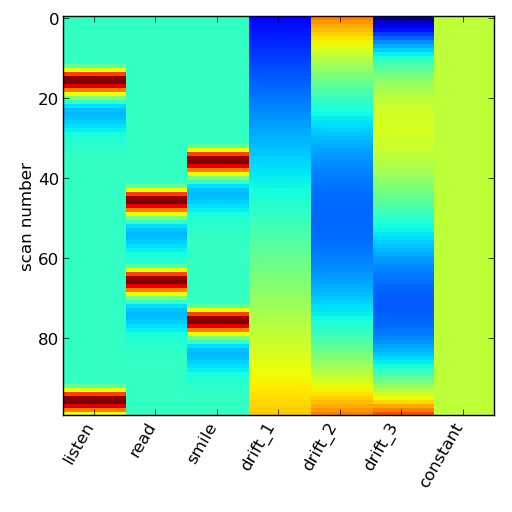
\includegraphics[width=.9\linewidth]{dmtx.png}
\caption{ Result of listing 1: the design matrix contains columns that
  contains the ideal reponse to input stimuli and a basis of
  polynomial function to model temporal drifts.}
\end{figure}


General Linear Model fitting consists then in estimating the brain
responses associated with the columns of design matrix.
%
The fit consists in a weighted least-square fit to estimate the model
parameters and a variance-covariance matrix parametrized by two
parameters: the amount of noise variance in the voxel time course and
the lag-1 autocorrelation of the noise \cite{Bullmore1996}. 
%
The model and covariance parameters are estimated in an alternate
optimization scheme.
%
The corresponding interface is relatively simple, as the user simply
needs to provide the design matrix and the data matrix. 
%
It yields a class that contains summary statistics (estimated effects
and their covariance matrix) that can be used for durther
investiagtion; the standard way of exploiting this output consists in
specifying a linear combination of the regressors and test the
signifiance in signed (t-) or unsigned (F-test)
%


\subsection{Group analysis and statistics}



\subsection{Cluster-level analysis}



\subsection{Parcel-based Bayesian analysis}

A weakness of conventional mass-univariate group analysis is that it
relies on averaging unperfectly aligned multi-subject data, thereby
mixing signals from potentially different functional
areas. Cluster-level inference can be used to mitigate this problem,
but comes at the price of sacrificied localization power. NIPY
implements an alternative group inference method using a hierarchical
statistical model that explicititly incorporates spatial uncertainty
in the standard space, and performs an approximate Bayesian inference
on group effects assumed to be piecewise constant within the brain
according to a given, user-supplied parcellation
\citep{keller:sinica:08,keller:miccai:09}. 

The method is implemented by NIPY's {\tt ParcelAnalysis} class, which
typically runs in seconds owing to a fast expectation-propagation
scheme \citep{minka:techrep:05} used to carry out approximate
inference. An example of use is provided in
Figure~\ref{fig:parcel_group}, left panel, where we infer the effect
of changing the speaker for different sentences in an auditory fMRI
experiment from 15 {\em non-smoothed} first-level contrast images. We
use the AAL atlas \citep{tzourio:ni:02} as the underlying parcellation
in this example. The method highlights the inferior temporal gyri and
the left paracentral lobule as the regions with strongest
effects. Note that it is possible to switch off the localization
uncertainty model and replace it with conventional image smoothing, as
shown in the right panel of Figure~\ref{fig:parcel_group}. We then
obtain more regions with strong effects, but this likely is an
artefactual effect of smoothing.

\begin{figure}
\begin{center}
  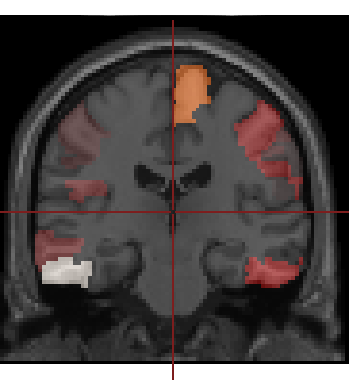
\includegraphics[width=0.23\textwidth]{parcel_group_analysis.png}
  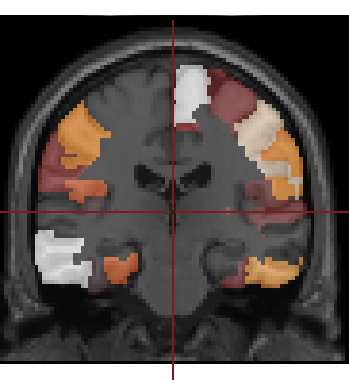
\includegraphics[width=0.23\textwidth]{parcel_group_analysis_naive.png}
\end{center}
\caption{Parcel-based Bayesian estimation of BOLD effects at
  population level for a speaker effect in an auditory fMRI
  experiment. Left, using a model of localization uncertainty in MNI
  space; right, using conventional image smoothing
  (FWHM=8mm). Brighter colors indicate larger estimated effects.}
\label{fig:parcel_group}
\end{figure}

\subsection{Brain Functional landmarks}
% Bertrand

\section{Visualization}
% Gael or Bertrand

\section{Conclusion}


\section*{Acknowledgments}
Whom do we need to acknowledge?

\section*{Disclosure/Conflict-of-Interest Statement}
Is it true that there are no conflicts of interest relating to this
work?


\section*{Formatting stuff}

To be removed later on.

This is to show how graphics (EPS) files are included. We use EPS for
speed. The first one is spread across both columns, and the second one
is just in a single column:

\begin{figure*}
%\centerline{\includegraphics[width=160mm]{Figures/Fig_4_cst_simplification_relabeled_triple.eps}}
\caption{This is the figure caption - and a label to refer to it in the text \label{Fig:big_picture}}

\end{figure*}

When we want to refer to this figure we use the label (see
Fig.~\ref{Fig:big_picture}).


Here are some displayed equations (see Eq.~\ref{eq:direct_flip_distance}):
\begin{eqnarray}
  d_{\textrm{direct}}(s, t) = d(s, t) & = & \frac{1}{K}\sum_{i=1}^{K}|s_{i}-t_{i}|,\nonumber\\
  d_{\textrm{flipped}}(s, t) & = & d(s,t^F) = d(s^F,t),\nonumber\\
  \textrm{MDF}(s, t) & = & \min(d_{\textrm{direct}}(s, t), d_{\textrm{flipped}}(s, t))\label{eq:direct_flip_distance}.
\end{eqnarray}

Inline mathematics goes like this: $\frac{1}{K}\sum_{i=1}^{K}|s_{i}-t_{i}|$

Here we have an example of a table (see Table~\ref{Table_1}).

\begin{table}[th] \processtable{QB centroids performance compared with
random subsets\label{Table_1}} {\begin{tabular}{rrrr} %\hline Thresholds &
Comparison & Coverage \% (s.d.) & Overlap (s.d.) \\ \hline
\multirow{2}{*}{$10$~mm/$10$~mm} & QB Centroids & 99.96 (0.007) & 2.44
(0.08)\\ & Random & 90.49 (0.41) & 6.16 (0.55)\\ \hline
\multirow{2}{*}{$20$~mm/$20$~mm} & QB Centroids & 99.99 (0.004) & 3.54
(0.18)\\ & Random & 95.86 (0.62) & 6.81 (0.93)\\ \hline
\end{tabular}}{}
\end{table}


%%\selectlanguage{british}%
\bibliographystyle{apalike2}
%\bibliographystyle{plainnat}
%\bibliographystyle{IEEEabrv, IEEEtran}
%\bibliographystyle{IEEEtran}
%\bibliographystyle{elsarticle-harv}
\selectlanguage{english}
\bibliography{nipy_paper}

\end{document}
